\documentclass[11pt,a4paper]{book}
\usepackage{titlesec}
\usepackage{setspace}
\usepackage{graphicx}
\usepackage{wrapfig}
\usepackage{color,soul}
\usepackage[customcolors,shade]{hf-tikz}
\usepackage{amsmath}
\usepackage{amssymb}
\usepackage{graphicx}
\usepackage{subfig}
\usepackage{sidecap}
\graphicspath{{/Users/giuliodilernia/Documents/Laboratory-Notes/Teoria_Lab2/images/}}

\renewcommand{\baselinestretch}{1.3} 

\titleformat{\chapter}[display]
 {\bfseries\Large}
  {\filright\MakeUppercase{\chaptertitlename} \Huge\thechapter}
  {1ex}
  {\titlerule\vspace{1ex}\filleft}
  [\vspace{1ex}\titlerule]

\begin{document}
\setcounter{chapter}{4}
\chapter{Maximum Likelihood e Minimi Quadrati}

\section{La Verosomiglianza - Likelihood}

Date N misure  $\{x_{i}\}_{i}^N$ queste si definiscono IID quando sono:
\begin{itemize}
\item \textbf{indipendenti:} l'esito di un campionamento non \`{e} influenzato da nessuno degli altri
\item \textbf{identicamente distribuiti:} Tutte le misure seguono la stessa funzione di distribuzione di pobabilit\`{a}
\end{itemize}
\begin{equation*}
		pdf_x(x,\underline{\theta}): R \rightarrow R^+
\end{equation*}

\noindent La funzione di probabilit\`{a} congiunta (joint-pdf) di N campionamenti IID \`{e} il prodotto delle singole probabilit\`{a} (poich\`{e} indipendenti tra loro):

\begin{equation*}
		pdf_{set}(x_1.....,x_N,\underline{\theta}) = \prod_{i}^N pdf_{x}(x_i,\underline{\theta_{t}})	
\end{equation*}

\noindent essa rappresenta la densit\`{a} di probabilit\`{a} da associare all'evento casuale consistente nell'estrarre un particolare set di dati, ed \`{e} una funzione definita su uno spazio N-dimensionale.\newline

\noindent Se si sostituisce al valore vero $\underline{\theta_{t}}$ il generico valore $\underline{\hat{\theta}}$ stimato dalle N misure e se esse vengono considerate non pi\`{u} variabili casuali, ma costanti che sono state determinate dalle operazioni di misura, la precedente funzione prende il nome di \textit{funzione di verosomiglianza} o \textbf{likelihood}.

\begin{equation*}
		 L(\underline{x},\underline{\hat{\theta}}) = \prod_{i}^N pdf_{x}(x_i,\underline{\hat{\theta}}) 
\end{equation*}


\noindent Rappresenta la densit\`{a} di probabilit\`{a} da associare all-evento casuale consistente nell'essere un certo $\underline{\hat{\theta}}$ il valore vero del nostro parametro, nell'ipotesi di avere gi\`{a} ottenuto un set di N misure.\newline

\noindent \`{E} possibile definire anche la \textbf{loglikelihood} ovvero:

\begin{equation*}
	 l(\underline{\theta})= \log(L(\underline{x},\underline{\hat{\theta}})) = \log(\prod_{i}^N pdf_{x}(x_i,\underline{\hat{\theta}})) = \sum_{i}^N \log(pdf_{x}(x_{i},\underline{\theta})
\end{equation*}

\section{Comportamento della likelihood}

\noindent Raccolte delle misure $\{x_{i}\}_i^N$ IID, la funzione di likelihood $L(\theta)$ restituisce la probabilit\`{a} che si aveva di raccogliere tale campione assunta la conoscenza del parametro $\theta$  (che per comodit\`{a} in questo capitolo assumiamo in una sola dimensione). 
\hspace{0.5in}

\begin{wrapfigure}{r}{0.\textwidth}
\centering

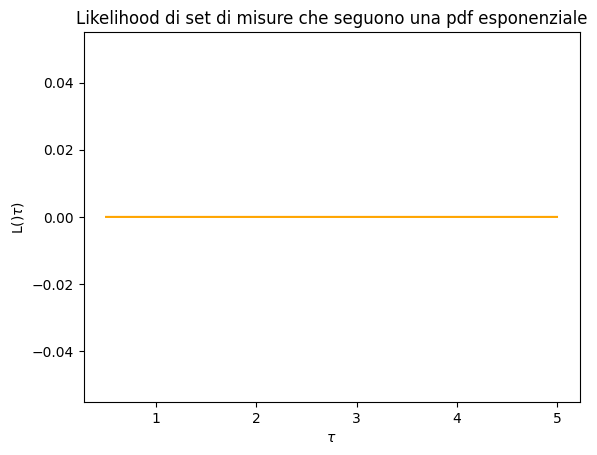
\includegraphics[scale = 0.4]{Like.png}	

\end{wrapfigure}

\noindent Se la $L(\theta)$ \`{e} all'incirca piatta vuol dire che  si ha la stessa probabilit\`{a} di ottenere un campionamento $\{x_1,....,x_N\}$ per ogni valore di $\theta$, ci\`{o} significa che i campionamenti non forniscono molte informazioni sul parametro $\theta$.  

\hspace{0.5in}


Se la $L(\theta)$ \`{e} una campana vuol dire si avr\`{a} una probabilit\`{a}:


\begin{wrapfigure}[5]{l}{0.5 \textwidth}

\vspace{-10pt}
\centering
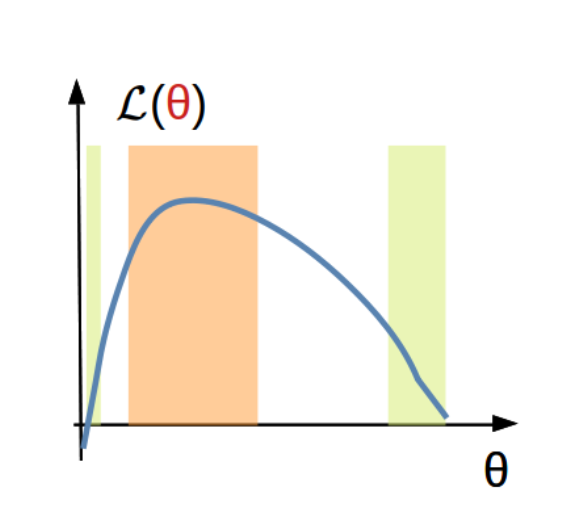
\includegraphics[width = 0.45 \textwidth]{loglike}	

\end{wrapfigure}

\noindent $\bullet \;$  Alta se il $\theta_{t}$ del campione \`{e} nell'area arancione in figura \\
\noindent $\bullet \;$ bassa se $\theta_{t}$ \`{e} nella regione verde \\
\noindent $\bullet \;$ massima se $\theta_{t}$ coincide con il massimo della funzione di likelihood \\
 
\noindent di aver raccolto il set di dati in esame. Dunque i campionamenti forniscono informazioni su $\theta$. Pi\`{u} \`{e} stretta la campana e pi\`{u} piccolo \`{e} il range dei valori che massimizzano la probabilit\`{a} di ottenere il campione raccolto. La larghezza della campana \`{e} legata all'incertezza con cui \`{e} possibile determinare il valore vero di $\theta$.
\newline

\noindent Quando definiamo una $pdf(x,\theta)$ senza conoscere $\theta$ si descrive un fascio di distribuzioni di probabilit\`{a} e dunque un'infinit\`{a} di modelli diversi. Cambiando la varianza di una distribuzione di cambia anche la funzione di likelihood.

\section{Minimum Variance Bound}

La funzione di likelihood $L(\theta)$ pu\`{o} essere utilizzata per misurare l'informazione che i campionamenti contengono relativamente al parametro $\theta$ che descrive il modello. L'informazione cos\`{i} ottenuta consente di valulatare la minima varianza  raggiungibile di uno stimatore di $\hat{\theta}$, ovvero dato un insieme di misure e un modello  esiste un limite inferiore  alla varianza raggiungibile.

\subsection{Informazione di Fischer}

Vogliamo costruire una metrica che $I ( \theta)$ che fornisca l'ammontare d'informazione contenuta in una variabile casuale osservabile x, relativamente a un parametro non osservabile $\theta$, da cui dipende la pdf(x). Tale funzione  prende il nome d'\textbf{informazione di Fischer}.

\begin{equation*}
		I(\theta) = E[(\frac{\partial}{\partial \theta}log(L(\theta)))^2] = -E[\frac{\partial^2}{\partial\theta^2}log(L(\theta)]
\end{equation*}

\noindent essa gode delle seguenti propriet\`{a}:

\begin{itemize}
	\item Associa un valore nullo se i dati sono irrilevanti per la stima di $\theta$.
	\item Aumenta al crescere della dimensione del campione ( purch\`{e} i dati siano rilevanti per la stima di $\theta)$.
	\item \`{E} legata alla precisione della stima: se l'informazione aumenta la varianza minima raggiungibile da uno stimatore $\hat{\theta}$ diminuisce.
\end{itemize}

\noindent Pi\`{u} i valori assunti dalla likelihood risultano essere sparpagliati peggiore \`{e} l'informazione che si ha a disposizione e dunque la precisione di stima di uno stimatore ne risentir\`{a} in egual modo. Viceversa pi\`{u} i valori risultano essere raggruppati in un certa regione di spazio e migliore sar\`{a} la precisione con cui si ottiene lo stimatore.

\subsection{Teorema di Rao - Cram\'{e}r}

Per uno stimatore $\hat{\theta}(x)$ consistente, bias $b_n(\hat{\theta})$, $V[\hat{\theta}] < \infty$ e non dipendente da x, definito su un dominio $\Omega_{\theta}$ si ha che il \textbf{MVB (Minimum Variance Bound)} definisce una relazione tra la varianza di un qualsiasi stimato $\hat{\theta}$ e la likelihood $L(\underline{X},\theta)$ nel seguente modo:

\begin{equation}
	V[\hat{\theta}] \geq \frac{(1-\frac{\partial}{\partial \theta}b_n(\theta))^2}{E[(\frac{\partial}{\partial \theta}log(L(\theta)))^2]} = V[\hat{\theta}]_{min}
\end{equation}
\newline
\noindent Al numeratore si ha una quantit\`{a} che dipende dallo specifico stimatore $\hat{\theta}$, ma solo se questo \`{e} biased, mentre a denominatore si ha l'informazione di Fischer, dunque una quantit\`{a} che non dipende dallo specifico stimatore ma solo da modello e dati.
\newline

\noindent Diciamo che uno stimatore \`{e} \textbf{efficiente} se la grandezza:

\begin{equation}
	\xi(\hat{\theta}) = \frac{V[\hat{\theta}]_{min}}{V[\hat{\theta}]} = 1
\end{equation}
	
\section{Maximum Likelihood}

Considerato un campione di N misure IID, si definiscono stimatori di \textbf{Maximum Likelihood (ML)} dei parametri quei valori che massimizzano la funzione di likelihood. Data una likelihood differenziabile rispetto $\underline{\theta}$ e il cui punto di massimo non \`{e} ai margini del range dei parametri, gli stimatori $\underline{\hat{\theta}}$ sono dati dalla soluzione delle equazioni differenziali:

\begin{equation}
\frac{\partial L}{\partial \theta_{i}}=0 \;\;\; i = 1,....,N
\end{equation}

\noindent Se esiste pi\`{u} di un massimo, viene considerato il maggiore. \newline

\noindent Con questa definizione di ML si considera il valore dello stimatore in corrispondenza del quale la probabilit\`{a} associata al campionamento \`{e} la massima possibile.

\noindent Le propriet\`{a} degli stimatori ottenute con il metodo di ML valgono asintoticamente, ovvero con un numero sufficientemente elevato di misure. Alcune \textbf{propriet\`{a} notevoli} sono:

\begin{enumerate}
	\item Consistente
	\item Asintoticamente efficiente
	\item Asintoticamente non distorto
	\item Propriet\`{a} d'invarianza: $\hat{\theta}_{ML}$ stimatore di $\theta_{t} \Rightarrow g(\hat{\theta}_{ML})$ \`{e} stimatore di $g(\theta_{t})$.
\end{enumerate}

\subsection*{Esempio propriet\`{a} d'invarianza}

Consideriamo la distribuzione esponenziale $f(x,\tau) = \frac{1}{\tau}e^{\frac{-t}{\tau}}$ e si abbiamo N misure IID la likelihood rispetto a $\tau$ \`{e} $L(\tau) = \prod_{i}^N \frac{1}{\tau}e^{\frac{-t_{i}}{\tau}}$.
\newline

\noindent Applichiamo il metodo di ML alla loglikelihood di $\tau$, dunque si ha che:

\begin{equation*}
		\sum_{i}^N(-\frac{1}{\tau}+ \frac{t_{i}}{\tau^2}) = 0 \iff N = \sum_{i}^N \frac{t_{i}}{\tau} \iff \tau_{ML} = \frac{1}{N} \sum_{i}^Nt_{i}
\end{equation*}

\noindent Posto $\lambda(\tau) = \frac{1}{\tau}$ possiamo riscrivere la pdf come $f(x,\lambda)= \lambda e^{-\lambda t}$ data la sostituzione vogliamo verificare che $\lambda(\tau_{ML}) = \frac{1}{\tau_{ML}}$.\newline


\noindent Dim.

\begin{equation*}
		\frac{\partial l}{\partial \theta} = 0 \iff \sum_{i}^N(\frac{1}{\lambda} - t_{i}) = 0 \iff \frac{N}{\lambda} = \sum_{i}^N t_{i} \iff \lambda = \frac{1}{\tau}
\end{equation*}

\noindent Se si dimostra che $\hat{\tau}$ \`{e} uno stimatore non distorto, \`{e} anche vero che $\hat{\lambda}$ \`{e} anch`esso non distorto ? \newline

Poich\`{e} la relazione $\hat{\lambda}(\hat{\tau})$ pu\`{o} essere non lineare non \`{e} detto che anche $\hat{\lambda}$ sia non distorto. 

\noindent Si pu\`{o} dimostrare che $\hat{\lambda}$ \`{e} uno stimatore distorto di $\lambda$ e dunque solo asintoticamente non lo \`{e}.

\section{Varianza dello stimatore di ML - Metodo Grafico}

Espandiamo fino al secondo ordine con un polinomio di Taylor la loglikelihood in un'intorno del parametro $\hat{\theta}$ ottenuto con il metodo di ML.

\begin{equation}
	log(L(\theta)) \approx log(L(\hat{\theta})) + \frac{1}{2}\frac{d^2}{d\theta^2}(log(L(\theta))\vert_{\theta = \hat{\theta}} (\theta - \hat{\theta})^2
\end{equation}

\noindent Se assumiamo che lo stimatore sia unbiased (il che per le propriet\`{a} precedente asintoticamente pu\`{o} esserlo) ed efficiente si ha dal teorema di Rao-Cramer che il secondo addendo \`{e} equivalente a:

\begin{equation*}
		\frac{d^2}{d\theta^2}(log(L(\theta))\vert_{\theta = \hat{\theta}} = - \frac{1}{\sigma_{\hat{\theta}_{ML}}}
\end{equation*}

\noindent E dunque possiamo riscrivere l'equazione (8.6) come:


\begin{equation}
	log(L(\theta)) \approx log(L(\hat{\theta})) -\frac{1}{2\sigma_{\hat{\theta}_{ML}}} (\theta - \hat{\theta})^2
\end{equation}

\noindent Consideriamo un cambio di variabile da $\hat{\theta}$ a $\hat{\theta}\pm \sigma_{\hat{\theta}}$ dunque possiamo riscrive la (8.7) come:

\begin{equation}
	log(L(\hat{\theta}\pm \sigma_{\hat{\theta}}) = log(L(\hat{\theta})) - \frac{1}{2}
\end{equation}

\noindent dunque da tale cambia di variabile si ha che la loglikelihood diminuisce della met\`{a} del suo valore di massimo. Si pu\`{o} dimostrare che la funzione di loglikelihood diventa una parabola (e la funzione di likelihood diventa una Gaussiana) per valori grandi del campione. Anche se la log(L) non \`{e} parabolica si pu\`{o} utilizzare l'equazione (8.8) come la definizione di errore statistico. Determinando i punti d'intersezione con quanto definito in (8.8) si ottiene una stima della varianza dello stimatore $\hat{\theta}$ usando il metodo di ML.

 
\begin{figure}[!ht]
\vspace{0.2in}
\includegraphics[scale = 0.32]{grafico}	
\centering
\vspace{0.2in}
\caption{funzione di loglikelihood, stima della varianza}
\end{figure}

\noindent Con un numero finito di misure l($\theta$) non \`{e} simmetrico e al crescere del numero di misure la forma funzionale assume un aspetto parabolico. Per simmetria la likelihood L($\theta$) diventa una Gaussiana.

 
\begin{figure}[!ht]
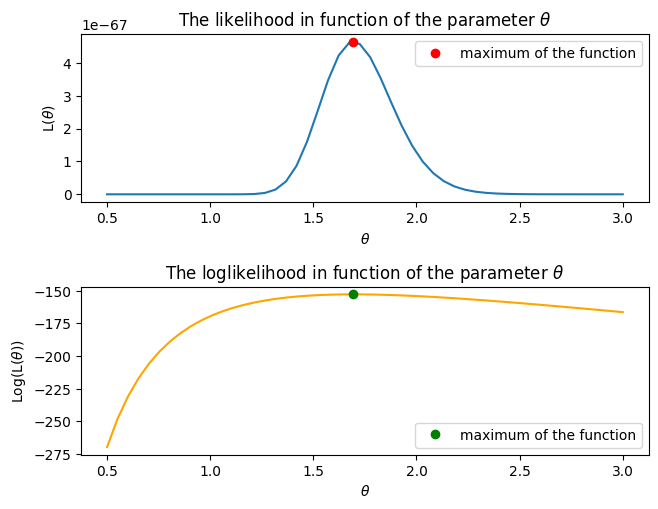
\includegraphics[scale = 0.45]{asinto}	
\centering
\caption{likelihood per un campione di 800 misure}
\end{figure}

\section{Extended likelihood}

Consideriamo una variabile aleatoria x distribuita secondo una pfd f(x,$\underline{\theta})$, dove i parametri $\underline{\theta}$ non li conosciamo e ipotizziamo di avere un campione di N misure $\{x_1,....,x_N\}$. Spesso si ha che il numero di osservazioni n del campione \`{e} una variabile aleatoria che segue una pdf Poissoniana con frequenza media $\lambda$. Il risultato di un'esperimento pu\`{o} essere definito dalla variabile n (che \`{e} la dimensione del campione) e dalle n misure raccolte $\{x_1,...,x_n\}.$ \newline
Dunque possiamo definire la likelihood dei parametri $\underline{\theta}$, dato un numero di venti medio $\lambda$ rispetto ad un campione di n misure.

\begin{equation}
	L(\lambda,\theta) = \dfrac{\lambda^{-n}}{n!}e^{-\lambda} \prod_{i=1}^nf(x_i,\underline{\theta}) = \dfrac{e^-{\lambda}}{n!} \prod_{i=1}^{n} \lambda_{i}f(x_i,\underline{\theta})
\end{equation}
Tale funzione prende il nome di \textbf{extended likelihood.}

\section{Varianza di uno stimatore per pi\`{u} parametri}

La varianza di $V[\hat{\theta}]$ di un vettore di parametri \`{e} definita dalla matrice di covarianza dove le sue componenti sono date da:

\begin{equation}
	V_{ij} = \Big[ - \dfrac{\partial^2}{\partial \theta_i \partial \theta_j}l(\hat{\theta}) \Big]^{-1} \quad \text{per} \quad i,j = 1,...,n
\end{equation}
dove i termini per $i \neq j$ sono dati da $Cov[\theta_i,\theta_j]$.
\section{Intervallo di confidenza}

Si \`{e} costruito uno stimatore $\hat{\theta}$ per un parametro $\theta$ che \`{e} una variabile aleatoria di conseguenza esiste una distribuzione pdf($\hat{\theta}$) che \`{e} caratterizzata da una media E[$\hat{\theta}$] e una varianza V[$\hat{\theta}$]. La \textbf{stima} \`{e} il valore che lo stimatore assume in corrispondenza di un campione di dati e lo definiamo $\hat{\theta}^*$.\newline

\noindent L'\textbf{intervallo di confidenza} \`{e} solitamente indicato come:
\begin{equation}
	\hat{\theta}^* \pm \sigma \quad \text{oppure} \quad \hat{\theta}^* \; \begin{matrix}
		+\sigma_1 \\ - \sigma_1
	\end{matrix}
\end{equation}
la seconda notazione viene usata quando l'intervallo \`{e} asimmetrico. \newline
\begin{wrapfigure}{r}{0.5 \textwidth}

\vspace{-10pt}
\centering
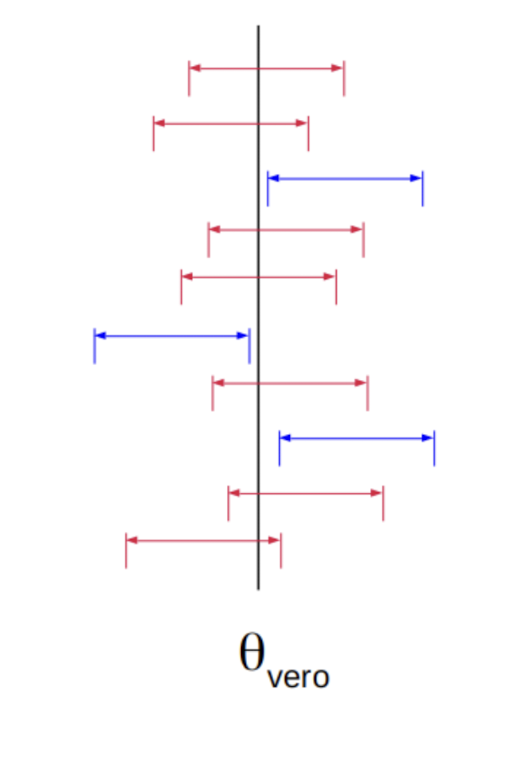
\includegraphics[width = 0.4 \textwidth]{interval}	

\end{wrapfigure}
In generale il risultato della stima \`{e} un intervallo [a,b], poich\`{e} \`{e} una variabile aleatoria si ha che gli estremanti sono variabili aleatorie e dunque per diversi campioni si hanno diversi intervalli di confidenza. A ciascun intervallo viene associata una probabilit\`{a} (\textbf{livello di confidenza}) che misura quanto \`{e} buona la stima del valore vero.

\begin{equation*}
	P(\theta_t \in [a,b])
\end{equation*}
dove essa rappresenta la frazione delle volte in cui ripetendo l'esperimento, la stima restituisce un intervallo che contiene il valore vero.\newline

In generale si vuole trovare un metodo che individui un intervallo [a,b] tale per cui la probabilit\`{a} che $\theta_t \in [a,b]$ sia pari a un certo valore $\beta$ detto \textbf{livello di confidenza}. Un intervallo di confidenza cos\`{i} definito prende il nome di \textbf{intervallo di condifenza di Neyman}. Un intervallo particolare \`{e} quello dato da $[\hat{\theta}^* - \sigma, \hat{\theta}^* + \sigma]$ e si definisce \textbf{intervallo centrale}.


\section{Metodo dei minimi quadrati}
Si parte da un modello $y = f(x,\underline{\theta})$ che definisce una relazione tra due grandezze fisiche x ed y e che dipende da N parametri $\underline{\theta}$, ipotizziamo di avere un campione di misure formato da punti $\{(x_i,y_i)\}_{i}^N$ ciascuno di essi segue una pdf(x) e una pdf(y) di conseguenza sono variabili aleatorie che hanno una loro incertezza $\sigma_x$ e $\sigma_y$. Vogliamo trovare un metodo che ci permetta di stimare i parametri ignoti partendo dai dati sperimentali. Tale metodo prende il nome di \textbf{interpolazione} o \textbf{fit} dei dati. Per semplicit\`{a} consideriamo il caso il cui l'incertezza sulle misure x sia trascurabile.

\subsection{Funzionale $Q^2$}

\noindent Partiamo considerando solo la variabile aleatoria x  e ci domandiamo per 
\begin{wrapfigure}{r}{0.5 \textwidth}
\vspace{-10pt}
\centering
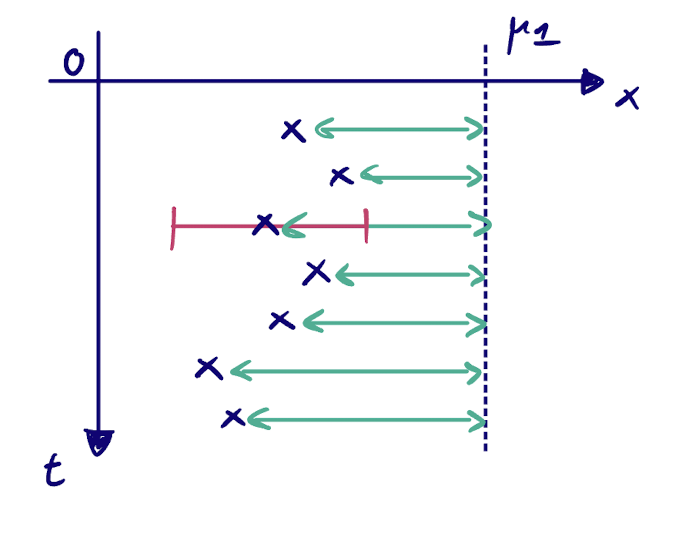
\includegraphics[width = 0.4 \textwidth]{q2}	
\end{wrapfigure}
quali valori del campione, si minimizza la distanza dalla media della popolazione $E[x] = \mu$; per rispondere a tale domanda definiamo la misura della distanza definendo un funzionale:
\newline

\begin{equation}
	Q^2\Big(\{x_i\}_1^N,\mu \Big) = \dfrac{1}{N}\sum_{i=1}^N\dfrac{(x_i - \mu)^2}{\sigma_i^2}
\end{equation}
\newline
Dunque ciascuna distanza \`{e} normalizzata alla larghezza della $pdf(x_i)$ e quindi tiene conto delle fluttuazioni statistiche di quel determinato campionamento.\newline
 Per determinare il  parametro cerchiamo quel valore $\hat{\mu}_{MQ}$ per cui $Q^2$ ammette un minimo assoluto nello spazio dei parametri (che nel nostro caso ha dimensione 1):

\begin{equation}
	\dfrac{d}{d\mu}Q^2 \Big(\{x_i\}_1^N, \mu \Big) = 0
\end{equation}
 

\subsection{Valore di aspettazione di $\hat{\mu}_{MQ}$}

Derivando la funzione di $Q^2$ si ha:

\begin{equation*}
	\dfrac{d}{d\mu}Q^2 = -2 \sum_{i=1}^N \dfrac{(x-\hat{\mu}_{MQ})}{\sigma_i^2} = 0 \iff  \hat{\mu}_{MQ} = \dfrac{\sum_{i=1}^N \frac{x_i}{\sigma_i^2}}{\sum_{i=1}^N \frac{1}{\sigma^2_i}}= \overline{x}
\end{equation*}

\noindent dunque per un campione di N misure la stima del valore atteso della popolazione coincide con la media aritmetica pesata del campione.

\subsection{Varianza dello stimatore $\hat{\mu}_{MQ}$}

Consideriamo $\hat{\mu}_{MQ} = \phi(x_1,....,x_N)$ e che il campione sia costituito da misure statisticamente indipendenti rispetto la variabile aleatoria x, la varianza dello stimatore sar\'{a} data da:

\begin{equation*}
	V[\hat{\mu}_{MQ}] = \sum_{i=1}^{N} \Big (\dfrac{\partial \phi}{\partial x_{i}} \Big)^2 \sigma_i^2 = \Big [\sum_{i=1}^N \frac{1}{\sigma^2_i} \Big ]^{-2} \sum_{i=1}^N \Big(\dfrac{1}{\sigma^2}\Big)^2 \sigma_i^2 = \dfrac{1}{\sum_{i=1}^N \frac{1}{\sigma^2_i}} < \sigma_i^2 \quad \forall i  
\end{equation*}
L'incertezza \`{e} dominata dalle misure con le $\sigma_{i}$ pi\`{u} piccole.

\section{Varianza di un stimatore usando i MQ - Metodo grafico}

Con il metodo di maximum likelihood si sono cercati i valori dei parametri che rendevano massima la probabilit\`{a}, dato un modello, di osservare i dati campionati. Con il metodo dei minimi quadrati invece si ceca il valore dei parametri che rende minima la distanza tra i dati campionati e il modello. Quando le $pdf(x_i)$ sono Gaussiane i due stimatori coincidono.

\begin{equation*}
	L(\hat{\theta}) = \prod_{i=1}^N \dfrac{1}{\sqrt{2\pi}\sigma_i}\exp{\Big [-\frac{ (x_i-\hat{\theta})^2}{2 \sigma_i^2} \Big]} = cost \cdot e^{-\frac{Q^2}{2}}
\end{equation*}
se passiamo alla loglikelihood

\begin{equation*}
	\log(L(\hat{\theta})) = \log(\text{cost}) - \dfrac{Q^2(\hat{\theta)}}{2}
\end{equation*}
Stimando $\hat{\theta}$ con il metodo di Maximum Likelihood si ha

\begin{equation}
	\dfrac{\partial \log(L(\hat{\theta}))}{\partial \hat{\theta}} = - \dfrac{1}{2}\dfrac{\partial Q^2(\hat{\theta})}{\partial \hat{\theta}}
\end{equation}
Quandole misure seguono una pdf Gaussiana e lo stimatore $\hat{\theta}$ \`{e} efficiente e non distorto sappiamo che il MVB coincide con la varianza dello stimatore ottenuto con il metodo di ML.

\begin{equation}
	V[\hat{\theta}_{ML}] = - \dfrac{1}{\dfrac{\partial^2 \log(L(\theta))}{\partial \theta^2} \Big \vert_{\theta = \hat{\theta}_{ML}}} 
\end{equation}
Dalla relazione (5.12) possiamo riscrivere l'uguaglianza (5.13) come:

\begin{equation}
	V[\hat{\theta}_{MQ}] = \dfrac{2}{\dfrac{\partial^2Q^2(\theta)}{\partial \theta^2} \Big \vert_{\theta = \hat{\theta}_{MQ}}}
\end{equation}
Sviluppando con Taylor al secondo ordine la funzione $Q^2$ in un intorno di $\hat{\theta}_{MQ}$ si ha:

\begin{equation*}
	Q^2(\theta) \approx Q^2(\hat{\theta}_{MQ}) + \dfrac{1}{2}\dfrac{d^2 Q^2(\theta)}{d\theta^2}\Big \vert_{\theta = \hat{\theta}_{MQ}}(\theta - \hat{\theta}_{MQ})^2 = Q^2(\hat{\theta}_{MQ}) + \dfrac{(\theta - \hat{\theta}_{MQ})^2}{V[\theta]}
\end{equation*}
Effettuando un cambio di coordinate $\theta = \hat{\theta}_{MQ} \pm \sigma_{\hat{\theta}}$ si ha:
\begin{equation*}
	Q^2(\hat{\theta}_{MQ} \pm \sigma_{\hat{\theta}}) = Q^2(\hat{\theta}_{MQ}) + 1
\end{equation*}
\begin{wrapfigure}[8]{r}{0.5 \textwidth}
\centering
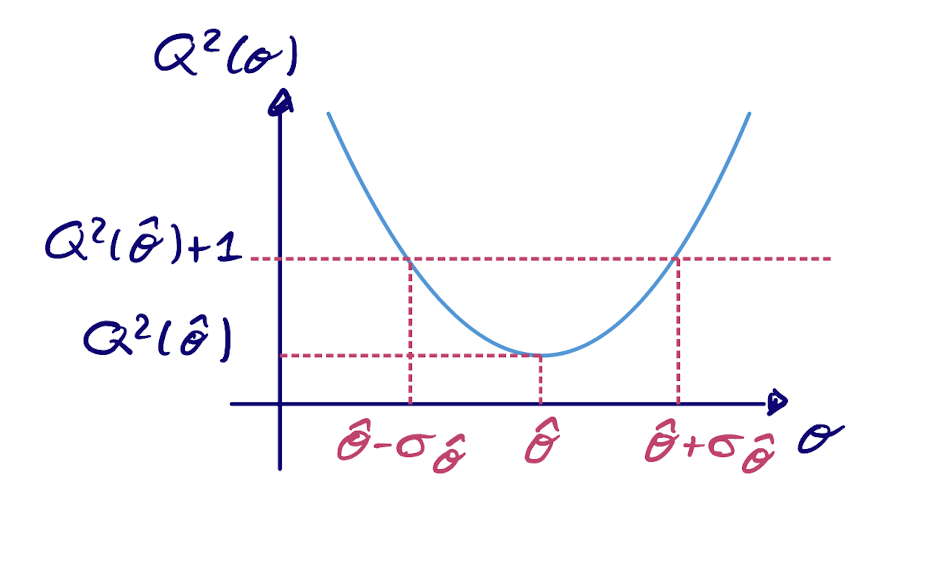
\includegraphics[width = 0.6 \textwidth]{graph}	

\end{wrapfigure}
\newline
Dunque considerando graficamente l'intersezione con $Q^2(\theta)$ si determinano $\hat{\theta}_{MQ} \pm \sigma_{\hat{\theta}}$. Poich\`{e} per ipotesi le misure $\{x_i\}_i^N$ seguono una distribuzione di probabilit\`{a} Gaussiana e sono IID si ha che $Q^2(\theta)$ segue la distribuzione di probabilit\`{a} del chi quadro $\chi^1(N-k)$ per E[$Q^2$] = N-k gradi di libert\`{a}. Se questo non avviene \`{e} perch\`{e}:
\begin{itemize}
	\item si \`{e} avuta una fluttuazione statistica sfavorevole
	\item il modello non descrive i dati
	\item il modello \`{e} corretto, ma i dati sono stati raccolti in modo errato
	\item il modello \`{e} corretto, ma le incertezze attribuite ai dati sono sbagliate (sono sopra o sottovalutate).
\end{itemize}

\section{Modelli lineari nei parametri}

Un modello si definisce \textbf{lineare} se due grandezza fisiche x ed y sono legate da una relazione lineare rispetto a parametr $\underline{\theta}$.

\begin{equation}
	y_{0}^{i} = \sum_{j = 1}^N \theta_{j}h_{j}(x_i)
\end{equation}
Assumiamo che l'incerteza sulla variabile x sia ininfluente, mentre y \`{e} una variabile aleatoria le cui misure sono IID con varianza $V[y_i] = \sigma_i^2$. Definiamo una variabile aleatoria asuiliaria $\epsilon$ che possiede la stessa distribuzione di probabilit\`{a} di y. Riscriviamo (5.15) come:

\begin{equation}
	y_i = \sum_{j = 1}^N \theta_{j}h_{j}(x_i) + \epsilon_i
\end{equation}
Assumiamo che per le $\epsilon$ valgano le seguenti propriet\'{a}:

\begin{equation*}
	E[\epsilon_i] = 0 \quad \quad V[\epsilon_i]= V[y_i] = \sigma_i^2
\end{equation*}
In questo modo la pdf(y) coincide con la pdf($\epsilon$). La variabile $\epsilon$ rappresenta l'errore statistico sulla misura, mentre le $y_0$ sono il valore vero della misura restituito dal modello.
\newline
Applichiamo il metodo dei minimi quadrati, andando a stimare quei valori dei parametri $\underline{\theta}$ che minimizzano la distanza tra il valore vero restituito dal modello lineare e i dati campionati sperimentalmente, pesando gli scarti quadratici rispetto la varianza delle distribuzioni di probabilit\`{a} delle singole $y_i$.

\newpage

 
\begin{figure}[ht]
\vspace{0.2in}
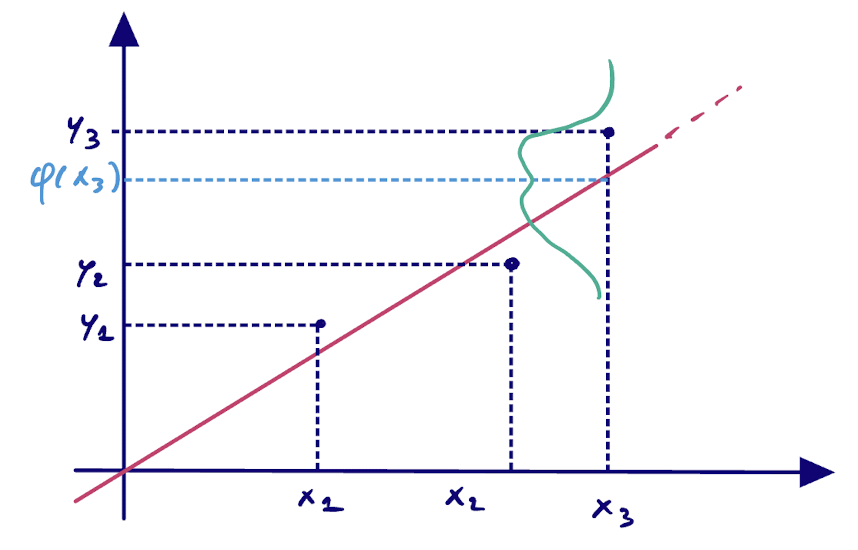
\includegraphics[scale = 0.5]{linear}	
\centering
\vspace{0.2in}
\caption{$\psi(x_3)$ rappresenta il valore vero della misura rispetto al modello, mentre $y_3$ il dato campionato su cui \`{e} presente un errore statistico.}
\end{figure}

\noindent Per farlo utilizziamo il funzionale $Q^2$ riscrivendolo come:

\begin{equation}
	Q^2 = \sum_{i=1}^N \dfrac{(y_i - y_0(x_i, \theta))^2}{\sigma_i^2} = \sum_{i=1}^N \dfrac{(y_i - \sum_{j=1}^N \theta_j h_j(x_i))^2}{\sigma_i^2} = \sum_{i=1}^N \dfrac{\epsilon_i}{\sigma^2_i} 
\end{equation}

\subsection{Stime dei parametri $\underline{\theta}$}

Per un vettore di parametri $\underline{\theta}$ di dimensione N, avremo un sistema di K equazioni:
\begin{align}
 \nabla Q^2(\underline{x},\underline{\theta}) =
	\begin{cases}
		\dfrac{\partial Q^{2}}{\partial \theta_{1}} = 0 \\
		\quad \vdots \\
		\dfrac{\partial Q^{2}}{\partial \theta_{n}} = 0 \\
	\end{cases} 
\end{align}
Per una singola riga si ha:
\begin{equation}
	\dfrac{\partial Q^{2}}{\partial\theta_{j}} = \sum_{i=1}^N \dfrac{-2}{\sigma^2_{j}} \Big ( \dfrac{y_i - \sum_{j=1}^N \theta_j h_j(x_i)}{\sigma_i} \Big )^2h_j(x_i) = 0 \quad \forall i = 1,...,N
\end{equation}
\newline
\noindent Per comodit\`{a} di esposizione riscriviamo l'espressione (5.16) in forma vettoriale:
\begin{equation}
	\underline{y} = H \underline{\theta} + \underline{\epsilon}
\end{equation}
ed essendo una modello a pi\`{u} parametri si ha la matrice di covarianza $V[\epsilon]$, possiamo considerare la matrice in funzione di $\epsilon$ poich\`{e} V[y] e $V[\epsilon]$ sono legate da una traslazione rigida e dunque risultano essere identiche. In generale tale matrice non \`{e} diagonale, ma poich\`{e} si \`{e} assunto che le misure siano IID la matrice \`{e} diagonale.
\begin{align*}
V[\epsilon] = 
\begin{bmatrix}
	\sigma_i^2 & \cdots\cdots & 0 \\
	\vdots & \ddots & \vdots \\
	0 & \cdots & \sigma_n^2
	\end{bmatrix}
\end{align*}
Riscrivendo $Q^2 = \underline{\epsilon}^TV^{-1}\underline{\epsilon}$ in forma matriciale e risolvendo il sistema (5.19) si stimano i parametri come:
\begin{equation}
	\underline{\hat{\theta }}_{MQ} = (H^TV^{-1}H)^{-1}\cdot H^TV^{-1}\underline{y}
\end{equation}
dove $V(\underline{\hat{\theta}}) = (H^TV^{-1}H)^{-1}$ dove nella matrice H \`{e} contenuta l'informazione delle misure.\newline
\noindent Resta da verificare che lo stimatore sia non distorto ovvero $E(\underline{\hat{\theta}}) = \underline{\theta}_t$:
\begin{equation*}
	E[\hat{\underline{\theta}}_{MQ}] = (H^TV^{-1}H)^{-1}\cdot H^TV^{-1}E[\underline{y}] = (H^TV^{-1}H)^{-1}\cdot (H^TV^{-1}H) \underline{\theta_t}
\end{equation*}
dove:
\begin{equation*}
	E[\underline{y}] = E[H \hat{\underline{\theta}} + \underline{\epsilon}] = E[H \hat{\underline{\theta}}] + E[\underline{\epsilon}] = H E[\hat{\underline{\theta}}] = H\underline{\theta}_t
\end{equation*}
duque lo stimatore ottenuto \`{e} non distorto.
\newline
A differenza del metodo di ML che gode di buone propriet\`{a} asintoticamente si ha che quello dei MQ le ha per un numero finito di misure.

\section{Sovrastima degli errori}

Ipotizziamo che le incertezze siano sovrastimate di un fatto $\alpha$ ovvero $\sigma_i^* = \alpha \cdot \sigma_i$, di conseguenza possiamo riscrivere la matrice di covarianza come:
\begin{align*}
W[y^*] = \alpha^2 \cdot  
\begin{bmatrix}
	\sigma_i^2 & \cdots\cdots & 0 \\
	\vdots & \ddots & \vdots \\
	0 & \cdots & \sigma_n^2
	\end{bmatrix}
	=\alpha^2 \cdot V[y]
\end{align*}
Se sostituiamo tale ipotesi all'interno dell'equazione (5.21) si ha:

\begin{equation}
	\underline{\hat{\theta }} = (H^TW^{-1}H)^{-1}\cdot H^TW^{-1}\underline{y} = \alpha^2 \cdot \dfrac{1}{\alpha^2} \cdot (H^TV^{-1}H)^{-1}\cdot H^TV^{-1}\underline{y} =  
\end{equation}
\begin{equation*}
	=(H^TV^{-1}H)^{-1}\cdot H^TV^{-1}\underline{y}
\end{equation*}
dunque la stima del parametro $\hat{\underline{\theta}}_{MQ}$ rimane invariata anche se si sono sovrastimate le incertezze. Quella che cambia \`{e} la varianza del parametro stimato infatti:
\begin{equation}
	V[\hat{\underline{\theta}}_{MQ}] = (H^{T}W^{-1}H)^{-1} = \alpha^2(H^{T}V^{-1}H)^{-1}
\end{equation}
e dunque viene sovrastimata di un fattore $\alpha^2$.

\subsection{Relazione tra il numero di parametri e il campione}

Se si hanno K parametri e campione di dimensione N dove K=N  si ha che:

\begin{itemize}
	\item il sistema ammette soluzione, e si ha una curva che passa per tutti i punti;
	\item se il sistema non ammette soluzione allora i dati falsificano il modello.
\end{itemize}

\subsection{Incertezze sulla variabile indipendente}

Nel caso in cui il modello sia lineare rispetto ai parametri, per esempio una retta $y(x,a,b) = a +bx$ e siano presenti delle incertezze sulla variabile indipendente x, si propaga l'errore sulle $y_i$ l'errore di $\sigma_{x_{i}}$ ottenendo un errore complessivo $\sigma_{i}^2 = \sigma_{y_{i}}^2 + b \sigma_{x_{i}}^2$ e dunque il funzionale $Q^2$ si riscrive come:
\begin{equation}
	Q^2 = \dfrac{1}{N}\sum_{i=1}^N\dfrac{(y_i - y)^2}{\sigma_{y_{i}}^2 + b \sigma_{x_{i}}^2}
\end{equation}
\subsection{Stima del fattore di sovrastima $\alpha$}

Ipotizziamo che gli $\underline{\epsilon}$ seguano una distribuzione di probabilit\`{a} Gaussiana e di avere N misure indipendenti allora il funzione $Q^2$ definito come l'ultima uguaglianza della (5.17) \`{e} segue la distribuzione di $\chi^2(N-K)$ per N-K gradi di libert\`{a} dove K \`{e} il numero di parametri da stimare. In forma matriciale possiamo riscriverlo rispetto alla matrice di sovrastima W come:

\begin{equation}
	\hat{Q^{2}} = \epsilon^TW^{-1}\epsilon = \dfrac{1}{\alpha^2} \cdot \epsilon^TW^{-1}\epsilon = \alpha ^{-2}\cdot Q^2
\end{equation}
Vogliamo determinare $\alpha^2$ affinch\`{e} $\hat{Q}_{min}^{2} = E[\hat{Q^2}] = N-K$ e dunque:

\begin{equation}
	\alpha^2 = \dfrac{\hat{Q}_{min}^{2}}{N-K}
\end{equation}

\begin{wrapfigure}{r}{0.\textwidth}
\centering

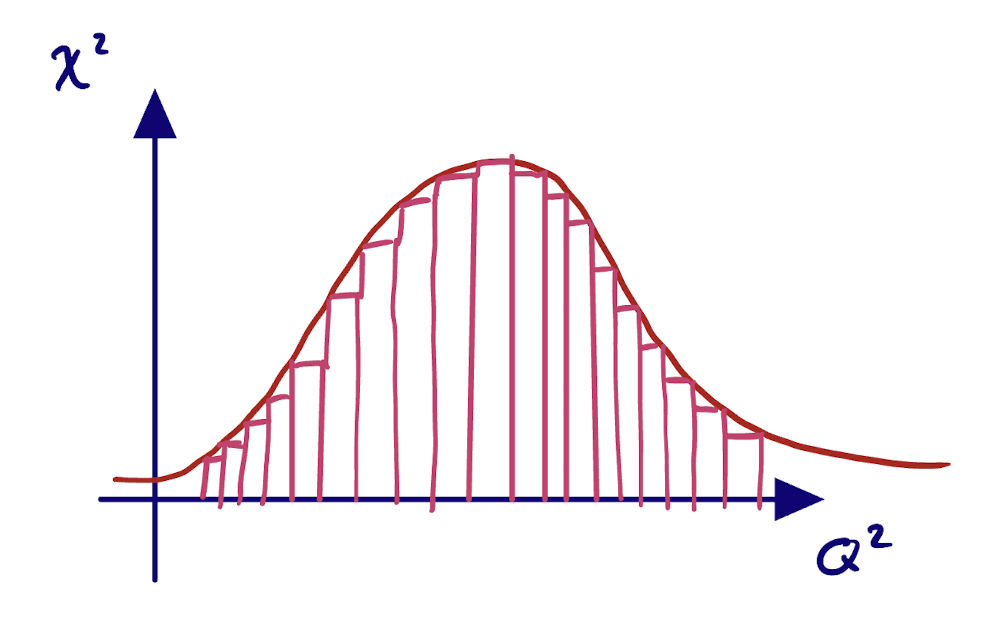
\includegraphics[scale = 0.36]{alpha}	

\end{wrapfigure}

\noindent Il fattore di scala cos\`{i} determinato non costituisce la sovrastima "reale" di cui si sono sbagliate le misure, poich\`{e} $\hat{Q^2}_{min}(\underline{x},\underline{\hat{\theta}}_{MQ})$ per $\underline{\hat{\theta}}_{MQ}$ fissato \`{e} anch'esso una variabile aleatoria  che segue la distribuzione di $\chi^2(N-K)$ di conseguenza la (5.26) stima un solo valore rispetto al campione a disposizione, ma $\alpha^2$ \`{e} una variabile aleatoria che segue la medesima distribuzione di $\hat{Q^2}_{min}(\underline{x},\underline{\hat{\theta}}_{MQ})$ e dunque per determinarlo bisogna ricostruire la distribuzione del $\chi^2$.

\section{Teorema di Gauss-Markov}
Si consideri un insieme di variabili aleatorie statisticamente indipendenti $\{(x_i,y_i)\}_i^N$ tali che sono legate tra loro da una relazione lineare rispetto ai parametri $y_i = \psi(x_i ,\underline{\theta}) + \epsilon_i$ dove $E[\epsilon_i] = 0$ e $V[\epsilon_i] $ finita $\forall i$ (propriet\`{a} di \textbf{omoschedasticit\`{a}}) ed inoltre $y_i$ indipendenti dai parametri $\underline{\theta} \Rightarrow$ si ha che lo stimatore $\underline{\hat{\theta}}$ ottenuto con il metodo dei minimi quadrati \`{e} non distorto e ha varianza minima fra tutti gli stimatori lineari.

\subsubsection{Osservazioni}

\begin{itemize}
	\item $\epsilon_{i}$ non \`{e} necessario che siano distribuite secondo una Gaussiana
	\item il teorema non ci dice che si \`{e} trovato lo stimatore pi\`{u} \textbf{efficiente} fra tutti gli stimatori possibili, ma sicuramente quello pi`{u} efficiente tra quelli lineari.
\end{itemize}  
\`{E} possibile trovare uno stimatore pi\`{u} efficiente per i parametri $\underline{\theta}$ per\`{o} dovremmo determinarlo con una funzione non lineare e ammesso che questa esista non \`{e} garantito che lo stimatore ottenuto sia non distorto.\newline
Gli stimatori descritti dal teorema di Gauss-Markov vengono definiti \textbf{B.L.U.E ( Best Linear Unbiased Estimator)}. 

\section{Interpolazione ed Estrapolazione}

\begin{wrapfigure}{l}{0.\textwidth}
\centering
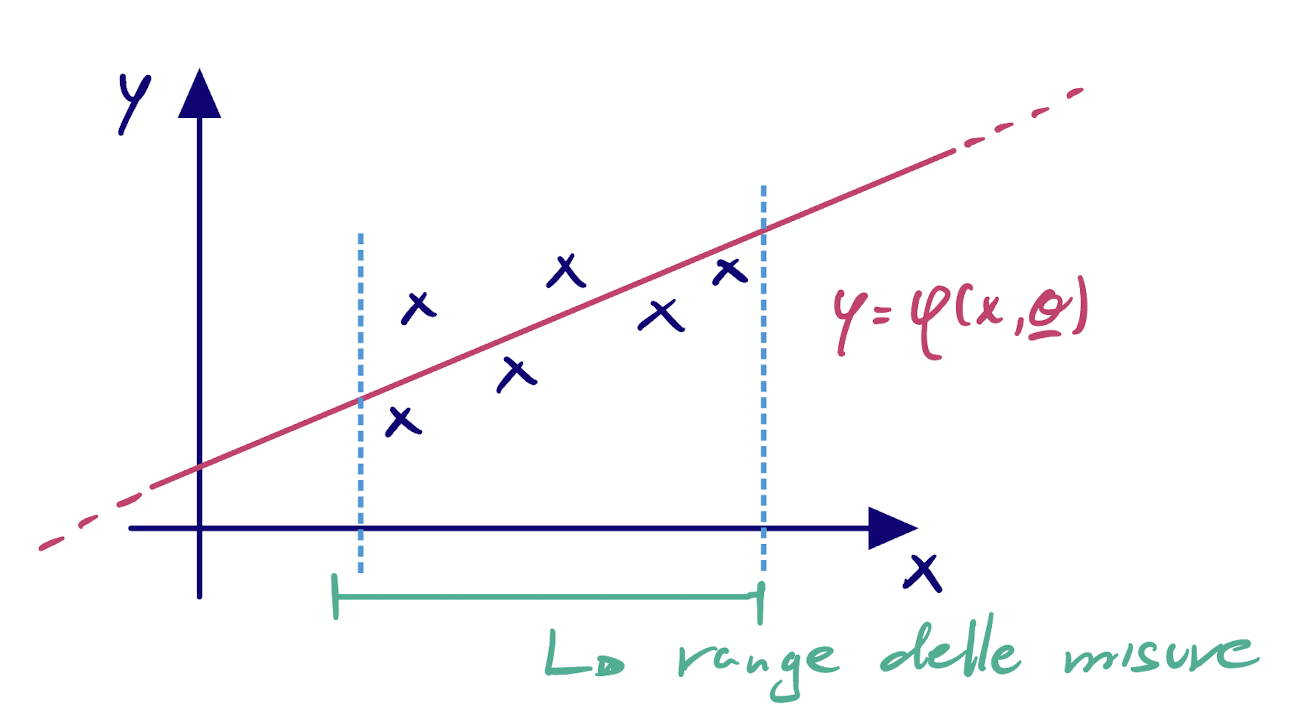
\includegraphics[scale = 0.35]{Estrapolazione}	
\end{wrapfigure}
Assumendo che i parametri $\underline{\theta}$ siano gi\`{a} stati determinati. \textbf{L'interpolazione} \`{e} la determinazione del valore di y mediante la funzione $\psi(x,\underline{\theta})$ per una misura x contenuta all'interno del range delle misure, ovvero l'intervallo contente i dati del campione. Si definisce \textbf{estrapolazione} il valore di y per qualsiasi altro valore di x non compreso all'interno del range delle misure definito sperimentalmente. Per una valore ottenuto da una retta di regressione lineare, l'errore \`{e} legato all'incertezza nella stima dei parametri di $\underline{\theta}$. Di conseguenza:

\begin{equation}
	V[y]_{i} = \nabla \psi(x,\underline{\theta})^T \cdot Cov[\underline{\hat{\theta}}_{MQ}] \cdot \nabla \psi(x,\underline{\theta}) 
\end{equation} 
Per esempio in un caso a due parametri si avr\`{a}:
\begin{align*}
V[y]_{i} = 
	\begin{bmatrix}
		\dfrac{\partial \psi}{\partial \theta_{1}} & & \dfrac{\partial \psi}{\partial \theta_{2}}  \\ 
	\end{bmatrix}
	\cdot 
	\begin{bmatrix}
		\sigma_{\theta_{1}}^2 & Cov(\theta_1,\theta_2) \\
		\\ 
		Cov(\theta_2,\theta_1) & \sigma_{\theta_{2}}^2 \\
	\end{bmatrix}
	\cdot 
	\begin{bmatrix}
		\dfrac{\partial \psi}{\partial \theta_{1}} \\
		\\
		\dfrac{\partial \psi}{\partial \theta_{2}} \\
	\end{bmatrix}
\end{align*}
che coincide con la formula di propagazione degli errori presente al capitolo 3. In generale l'errore aumenta allontanandosi dalla regione di campionamento ( quindi quando si passa dall'interpolazione all'estrapolazione).

\subsubsection{Esempio di fit lineare}

Consideriamo di avere un set di misure $\{(x_i,y_i) \}_{i}^N$ IID con incertezza $\sigma_{y_{i}}$ sulla variabile aleatoria y, e che il modello \`{e} quello di una retta y = a+bx, stimiamo i parametri a e b usando il metodo dei minimi quadrati. Avremo che:
\begin{align*}
\vec{\theta} =
	\begin{bmatrix}
		a \\
		b \\ 
	\end{bmatrix}
	\quad \quad \quad\vec{h}=
	\begin{bmatrix}
		1 \\
		x \\
	\end{bmatrix}
\end{align*}
e poich\`{e} le misure sono indipendenti tra loro, la matrice di covarianza \`{e} diagonale. Applicando il metodo dei MQ si stimano:
\begin{equation*}
	\hat{a} = \dfrac{1}{\sum_{i=1}^n \frac{1}{\sigma_i^2}}\sum_{i=1}^N \dfrac{y_i -\hat{b}x_i}{\sigma_i^2} = \overline{y} - \hat{b} \overline{x}
\end{equation*}

\begin{equation*}
	\hat{b} = \dfrac{1}{\sum_{i=1}^N \big (\frac{x_i}{\sigma_i} \big )^2}\sum_{i=1}^N \dfrac{y_ix_i -\hat{a}x_i}{\sigma_i^2} = \dfrac{\overline xy -\overline{x}\overline{y}}{\overline{x^2} - \overline{x}^2}
\end{equation*}
\newline
e le incertezze associate alle stime sono date dalla matrice di covarianza associate ai parametri:

\begin{align*}
V[\underline{\hat{\theta}}]=
	\begin{bmatrix}
		\sigma^2_{a} & Cov[a,b] \\
		Cov[b,a] & \sigma^2_{b} \\
	\end{bmatrix}
	= \textcolor{cyan}{\dfrac{\sigma^2}{N(\overline{x^2} - \overline{x}^2 )}} \cdot 
	\begin{bmatrix}
		\overline{x^2} & - \overline{x} \\
		- \overline{x} & 1 \\
	\end{bmatrix}
\end{align*} 

I termini in $\colorbox{cyan}{\phantom{b = \,}}$ viene definito \textbf{dispersione delle misure}. Si osserva che non necessariamente i parametri sono scorrelati tra loro. Pi\`{u} le msiure sono sparpagliate meigliore \`{e} la precisione con cui si stimano i parametri, poich\`{e} la banda che definisce le possibili rette che fittano i dati diventa pi\`{u} sottile, inoltre anche il numero di misure fornisce un contributo alla precisione con cui si determinano gli stimatori. \newline

\noindent Se calcoliamo il valore assunto dalla funzione in punto $x_0$ rispetto ai parametri $\hat{a}$ e $\hat{b}$ si ricava che l'errore su $y_0$ \`{e} dato da:

\begin{equation*}
	V[y_0] = \dfrac{\sigma^2}{N} \Big[ 1 + \dfrac{(x_0 - \overline{x})^2}{(\overline{x^2} - \overline{x}^2 )^2} \Big ]
\end{equation*}
Pi\`{u} $x_0$ si allontana da $\overline{x}$ pi\`{u} \`{e} grande la varianza su $y_0$.

\section{Fit d'istogrammi}
\begin{wrapfigure}{l}{0.\textwidth}
\centering
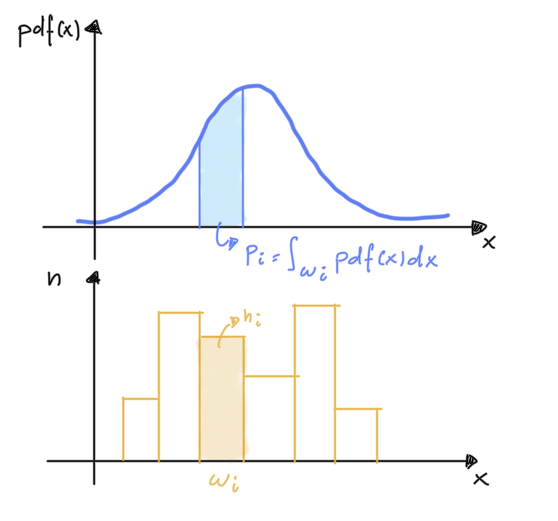
\includegraphics[scale = 0.34]{BinnedData}	
\end{wrapfigure}
Consideriamo un insieme di N misure $\{x_{i}\}_i^N$ IID che seguono la pdf $f(x_i,\vec{\theta}): \Omega \subseteq \mathbb{R} \rightarrow \mathbb{R}$, raccogliamo i dati in modo da dividere l'asse reale in k intervalli $\omega_j = [x_i,x_{i+1})$. tali che $\omega_j \cap \omega_i = \varnothing \quad \forall i,j$ e $\bigcup_{j=1}^k \omega_j = \Omega$. Tali intervalli vengono defini 'bin', per ciascuno di essi contiamo il numero di misure $n_j$ che cadono all'interno dell'intervallo. Complessivamente avremo che $\sum_{j=1}^N n_j = N$ numero totale di misure. Poich\`{e} le misure sono IID a ciascuna bin associamo una probabilit\`{a}:
\begin{equation*}
	p_j = \int_{\omega_j}pdf(x,\vec{\theta})dx \quad \forall j =1,...k
\end{equation*} 

\begin{wrapfigure}{r}{0.\textwidth}
\centering
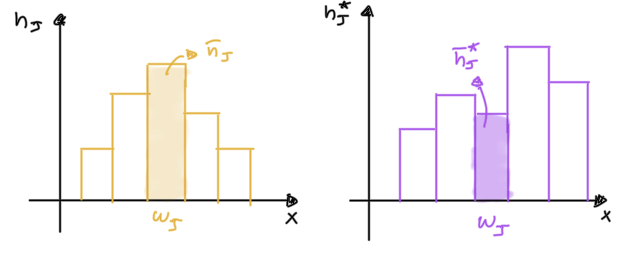
\includegraphics[scale = 0.32]{expbin}	
\end{wrapfigure}
Partendo dalla probabilit\`{a} associata a ciascun bin $\omega_j$ costruiamo un istogramma i cui conteggi attesi sono dati da $ E[n_{j}] = N \cdot p_j(\vec{\theta})$. Le misure di conteggio dell'istogramma definito dai dati del campione seguono una joint-pdf $pdf(n_1,...,n_k,p_1,...p_k)$ che definisce una distribuzione multinomiale. Per $p \rightarrow 0 $ le misure di conteggio sono statisticamente indipendenti tra loro di conseguenza la multinomiale pu\`{o} essere riscritta come prodotto di distribuzioni di probabilit\`{a} binomiali.
\begin{equation*}
	pdf(n_1,...,n_k,p_1,...,p_k) = \prod_{i=1}^kpdf(n_i,p_i)
\end{equation*}
Nel caso in cui il valore di aspettano del conteggio dei bin sia costante possiamo approssimare le singole pdf binomiali come delle Poissoniane dove $\lambda_{i}(\vec{\theta}) = N * p_i(\vec{\theta})$ rappresenta la frequenza media di eventi della distribuzione di Poisson di conseguenza la joint-pdf diventa :
\begin{equation*}
	\prod_{i=1}^kpdf(n_i,p_i) = \prod_{i=1}^k \dfrac{\lambda_i(\vec{\theta})^{n_{i}}}{n_{i}!}e^{-\lambda_{i}} = L(n_1,...,n_k,\theta)
\end{equation*}
Che coincide con la extended likelihood.\newline
Non solo si conosce la pdf associata ai dati ma anche il loro valore di aspettazione e varianza di conseguenza \`{e} possibile applicare il metodo di ML e dei MQ.
\subsubsection{Osservazioni}

Utilizzare le misure binnate ci permette di ridurre le dimensioni dei dati con cui si lavora, anche se si ha una perdita d'informazione questa viene bilanciata da una maggiore semplicit\`{a} e dalla possibilit\`{a} di usare differenti tecniche per la stima dei parametri, come per esempio quella di ML che per campioni molto grandi risulta essere da un punto di vista computazionale dispendiosa.

\subsection{Binned Data - Minimi Quadrati}

Applichiamo il metodo dei minimi quadrati confrontando i conteggi dell'istogramma dei dati con l'istogramma dei valori attesi. Dato un campione $\{x_i\}_i^N$ IID dopo averli rappresentati in un istogramma, associamo al valore atteso di conteggi per ciascun bin l'espressione:
\begin{equation*}
	\mu_i = E[n_j] = N \cdot \int_{\omega_j}pdf(x, \vec{\theta})dx = N \cdot p_j(\vec{\theta}) 
\end{equation*}
Scrivendo il funzionale $Q^2$ come:
\begin{equation*}
Q^2 = \sum_{i=1}^N\dfrac{(n_i - E[n_i])^2)}{V[n_i]}	 = \sum_{i=1}^N\dfrac{(n_i - Np_i(\vec{\theta}))^2)}{Np_i(\vec{\theta})} 
\end{equation*}
Assumendo che i conteggi $n_i$ seguano una pdf Poiss$(n_i,\mu_i)$ (la discussione che segue risulterebbe verificata ugualmente anche se le pdf fossero binomiali). Per $n_i \rightarrow \infty$ possiamo approssimare la poissoniana a una gaussiana con valore atteso e varianza pari a $\mu_i$ di conseguenza $Q^2$ dipendendo da variabili aleatorie distribuite secondo una gaussiana, ed essendo lui stesso una variabile casuale si ha che segue la distribuzioni di $\chi^2(k-s)$ dove s \`{e} il numero di parametri. Definiamo dunque il $\chi^2$ nella forma di \textbf{Neyman}:
\begin{equation}
	\chi^2_{Neyman} = \sum_{i=1}^N\dfrac{(n_i - \mu_i(\vec{\theta})^2)}{n_i} = \sum_{i=1}^N\dfrac{(O_i - E_i)^2}{O_i}
\end{equation} 
Dove per $n_i$ grande si \`{e} approssimata la $V[n_i] \approx n_i$. La necessit\`{a} di approssimare i dati a una Gaussiana e la varianza al numero di conteggi di un bin, \`{e} determinata dal fatto che cos\`{i} facendo il teorema di Gauss-Markov risulta soddisfatto poich\`{e} tra le ipotesi \`{e} necessario che i momenti non dipendano dai parametri. In conclusione si procede a minimizzare il $\chi^2_{Neyman}$ per determinare i parametri $\vec{\theta}$.

\subsubsection{Procedura di fit di un istogramma}
La procedura di fit di un istogramma con il metodo del $\chi^2$ di Neyman prevede quindi di:

\begin{itemize}
	\item verificare che sia rispetta l'ipotesi pdf($n_i$) gaussiana;
	\item associare a $n_i$ un errore $\sqrt{n_i}$
	\item calcolare per ogni valore del parametro $\theta_i$ i valori attesi $\mu_i$ dei conteggi in ciascun bin;
	\item minimizzare il $\chi^2_{Neyman}$ trovando il valore di $\theta$ per cui l'accordo valori misurati - valori attesi \`{e} il migliore;
	\item all'occorrenza effettuare un test del $\chi^2$
	\end{itemize}
	
	Se $N \cdot p_i$ \`{e} piccolo, la distribuzione binominale/poissoniana non \`{e} approssimabile a una Gaussiana. Ne consegue che $Q^2$ non \`{e} approssimabile ad un $\chi^2$ e la varianza non \'{e} aprossimabile con $n_i$, in questi casi il metodo dei MQ non \'{e} utilizzabile.
	
	\subsection{Binned Data - Maximum Likelihood}
	Fare il fit di un'istogramma quando non vale l'approssimazione Gaussiana prevede necessariamente l'utilizzo della binned Maximum Likelihood. Analogamente a quanto discusso a inizio sezione si procede a passare discretizzare il modello. Dove la funzione di likelihood associata al campione \`{e} data da
	
	\begin{equation*}
		L(n_1,...,n_k,\vec{\theta}) = \prod_{i}^k Bin(n_i,p_i(\vec{\theta},N)
	\end{equation*}
e si procede a massimizzare la funzione di likelihood:
\begin{equation*}
	\dfrac{\partial L(\vec{n},\vec{\theta})}{\partial \theta_j}= 0 \quad \quad \forall j=1,...,k
\end{equation*}
Ad un bin-size deve essere associata una probabilit\`{a} $p_{i}(\vec{\theta})$ piccola. Non \`{e} necessario che i bin abbiano tutti la stessa dimensione, possiamo sceglierle in modo che $N \cdot p_i$ sia grande e quindi valga l'approssimazione Gaussiana.\newline

L'operazione di binning, fa perdere informazione, questo si pu\`{o} riflettere sull'incertezza del parametro stimato , ma anche sulla capacit\`{a} di verificare che i dati siano ben descritti dal modello. In questi casi \`{e} utili studiare la dipendenza del risultato dal binning.



\end{document}
